\secrel{Разработка конструкции в САПР FreeCAD}\secdown


\includegraphics[height=0.5\textheight]{logo/FreeCAD.png}

\cp{https://ru.wikipedia.org/wiki/FreeCAD_(Juergen_Riegel\%27s)}
В среде специалистов ряда отраслей известна проблема создания полноценной САПР в
рамках OpenSource, и хотя FreeCAD ещё не является кандидатом на такую
«полноценность», этот продукт может рассматриваться как одна из попыток создания
базы для решения этой проблемы. Разработчик FreeCAD Юрген Ригель, работающий в
корпорации DaimlerChrysler, позиционирует свою программу как первый бесплатный
инструмент проектирования механики (сравнивая свой продукт с такими развитыми
проприетарными системами как CATIA версий 4 и 5, SolidWorks), созданный на
основе библиотеки \textbf{Open CASCADE}. Цель программы\ --- предоставить
базовый инструментарий этой библиотеки в интерактивном режиме.

Следует отметить, что имеет место ещё один программный продукт имеющий название
freeCAD, его разработчик\ --- Aik-Siong Koh, и он не связан с FreeCAD’ом Юргена
Ригеля.

\bigskip\cp{http://www.freecadweb.org/wiki/index.php?title=Getting\_started}
FreeCAD\ --- CAD/CAE приложение трёхмерного параметрического моделирования.
Оно в основном сделано для механического проектирования, но также может быть
использовано для любых других случаев, в которых вам нужно точно моделировать
трёхмерные объекты с контролем над историей моделирования.

FreeCAD все еще находится в ранней стадии разработки, так что, хотя он уже
предлагает Вам большой (и растущий) список функций, многого еще не хватает,
особенно если сравнивать его с коммерческими решениями, и вы можете не найти его
достаточно развитым для использования в производственной среде. Тем не менее,
есть быстрорастущее сообщество пользователей-энтузиастов, и вы уже можете найти
много примеров качественных проектов, разработанных с FreeCAD.

Как и все проекты с открытым исходным кодом, проект FreeCAD не единственый
способ работы обеспеченный Вам его разработчиками. Это во многом зависит от
роста его сообществу пользователей и разработчиком, доработки функций и
стабилизации кода (да здравствует исправление ошибок!). Так что не забывайте об
этом, когда начинаете использовать FreeCAD, если вам он нравится, вы можете
непосредственно влиять и помочь проекту!

\secrel{Установка}\secdown

\secrel{\win}

\menu{\winr>\url{http://www.freecadweb.org/}>Download>\win>\href{http://sourceforge.net/projects/free-cad/files/FreeCAD Windows/FreeCAD 0.14/}{\file{FreeCAD
0.14}}>\file{\ldots\_setup.exe}}

\menu{\file{FreeCAD 0.14.3700\_x86\_setup}>FreeCAD 0.14 License>I agree}

\menu{Distination Folder>\file{C:/FreeCAD}>Install>Completed>Close}

\menu{\winstart>Программы>FreeCAD 0.14>FreeCAD>\rms>Закрепить в панели задач}

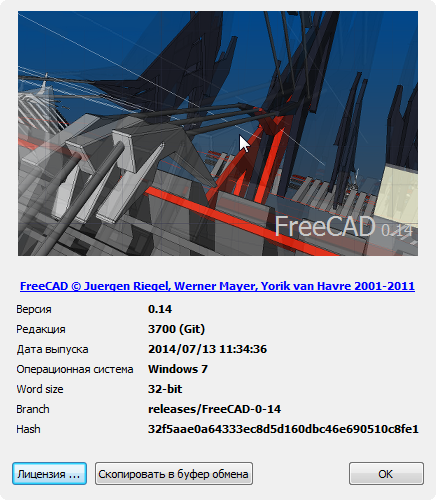
\includegraphics[height=0.8\textheight]{freecad/about.png}

\secrel{\linux}

\secup

% \secrel{Чертеж}
% 
% \secrel{Эскиз}
% 
% \secrel{Деталь}
% 
% \secrel{Сборка}
% 
% \secrel{Автогенерация конструкторской докуметации}
% 
% \secrel{Скрипты и пользовательские расширения}
% 

\secup